\documentclass{beamer}

\mode<presentation> {

\usetheme{Pittsburgh}


\setbeamertemplate{footline}[page number] 
}

\usepackage{caption}
\usepackage{graphicx}
\usepackage{booktabs}

%----------------------------------------------------------------------------------------

\title[Short title]{GC Content in Yeast} % The short title appears at the bottom of every slide, the full title is only on the title page

\author{Bo\v{z}ena Nevinskien\.{e}} % Your name
\institute[UCLA] % Your institution as it will appear on the bottom of every slide, may be shorthand to save space
{
Vilnius University, Systems Biology \\ % Your institution for the title page
\medskip
}
\date{November 18th, 2019} 

\begin{document}

\begin{frame}
\titlepage 
\end{frame}

%----------------------------------------------------------------------------------------

\begin{frame}
\frametitle{Goal of the study}
The purpose of this study is to determine if all yeast genes have the same GC content, and if not, why? 

Yeast's genome is approximately 12 Mb. 

GC content of \emph{Saccharomyces cerevisiae} should be 38.3\%.

3 random yeast strain were selected:
\begin{itemize}
\item EC9-8: found 8622 possible ORFS.
\item VL3: found 9859 possible ORFS.
\item YS9: found 8341 possible ORFS.
\end{itemize}
\end{frame}

%------------------------------------------------

\begin{frame}
\frametitle{Results - EC9-8}
EC9-8 is a haploid cadmium-resistant derivative of a yeast.

This yeast strain (EC9-8) had the highest number of outliers in GC ratio.
But on the average of G and C nucleotides in EC9-8 yeast strain's possible ORFS was approximately 39.94\%.
\begin{minipage}{0.4\textwidth}
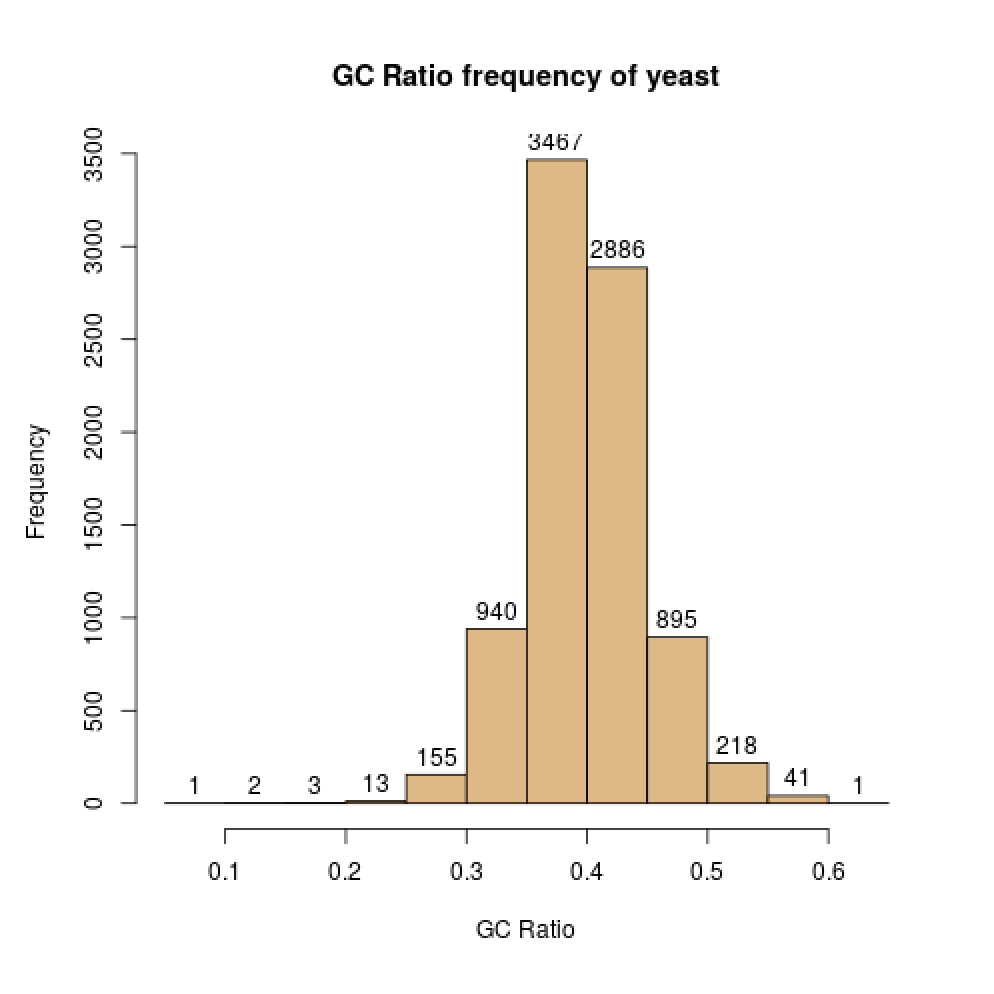
\includegraphics[width=60mm]{images/EC9-8_ASinica_2011_AGSJ01000000.eps}
\end{minipage}
\end{frame}

%------------------------------------------------

\begin{frame}
\frametitle{Results - VL3}

VL3 strain is most suited to the production of premium white wines.

The average of G and C nucleotides in this yeast strain's possible ORFS was approximately 39.67\%.
\begin{minipage}{0.5\textwidth}
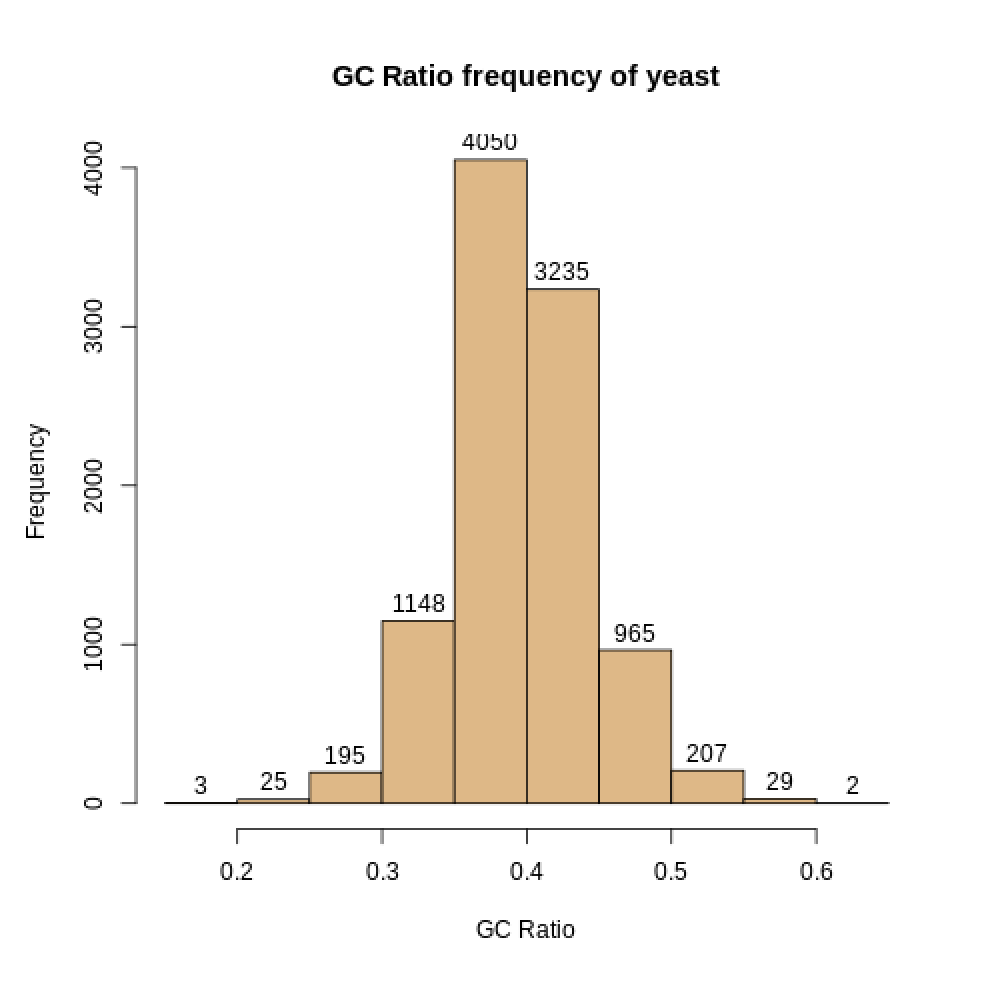
\includegraphics[width=60mm]{images/VL3_AWRI_2011_AEJS01000000.eps}
\end{minipage}
\end{frame}

%------------------------------------------------

\begin{frame}
\frametitle{Results - YS9}

YS9 is one of the Singapore's baking yeast strains.

The average of G and C nucleotides' ratio in EC9-8 yeast strain's possible ORFS was approximately 39.97\%.

\begin{minipage}{0.4\textwidth}
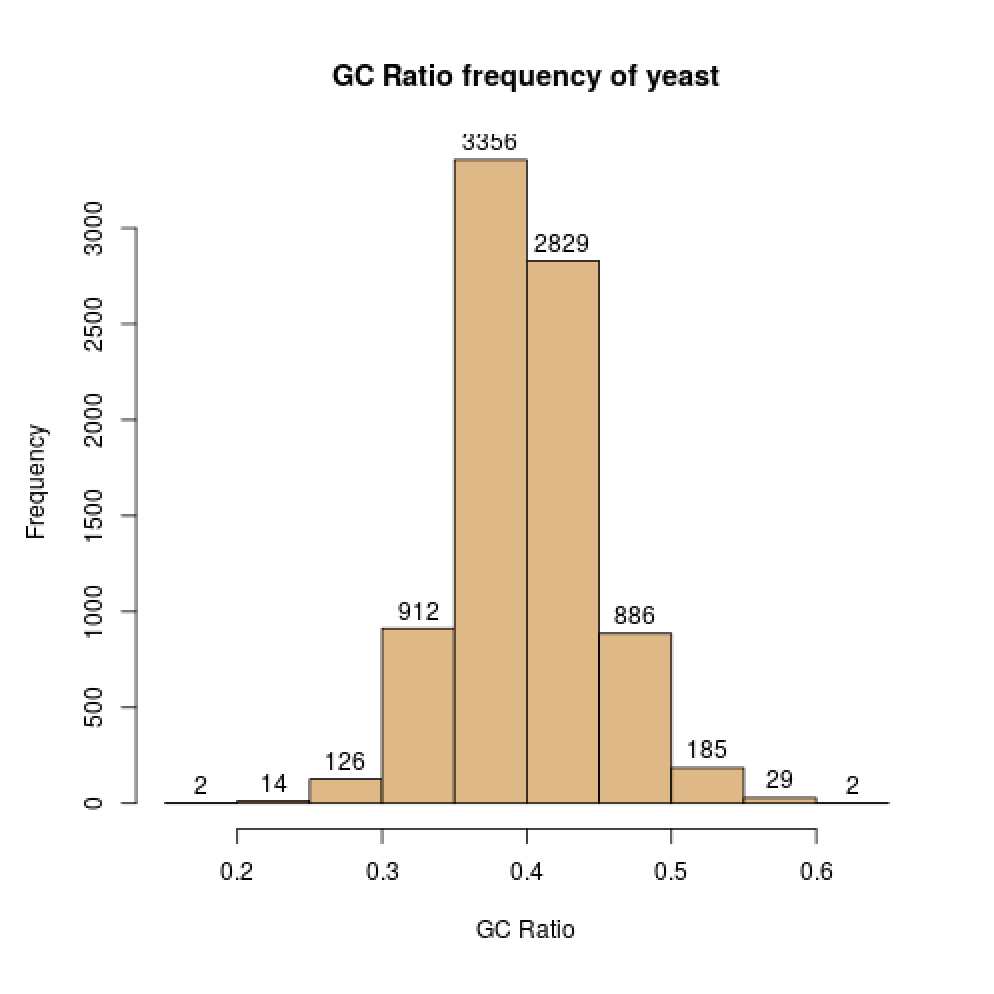
\includegraphics[width=60mm]{images/YS9_Stanford_2014_JRIB00000000.eps}
\end{minipage}
\end{frame}

%------------------------------------------------
\begin{frame}
\frametitle{Conclusions}

Overall in all 3 strains the mean ratio of G and C was 39.86\%.

Clearly, not all of yeast's genes contain the same GC number.

The most of possible open reading frames had GC ratios between 0.35 and 0.45. 

The GC-content of all three strains was similar, but not perfectly 38.3\% as it was predicted. This might be because we didn't analyse reverse complement ORFs.

\begin{minipage}{0.4\textwidth}
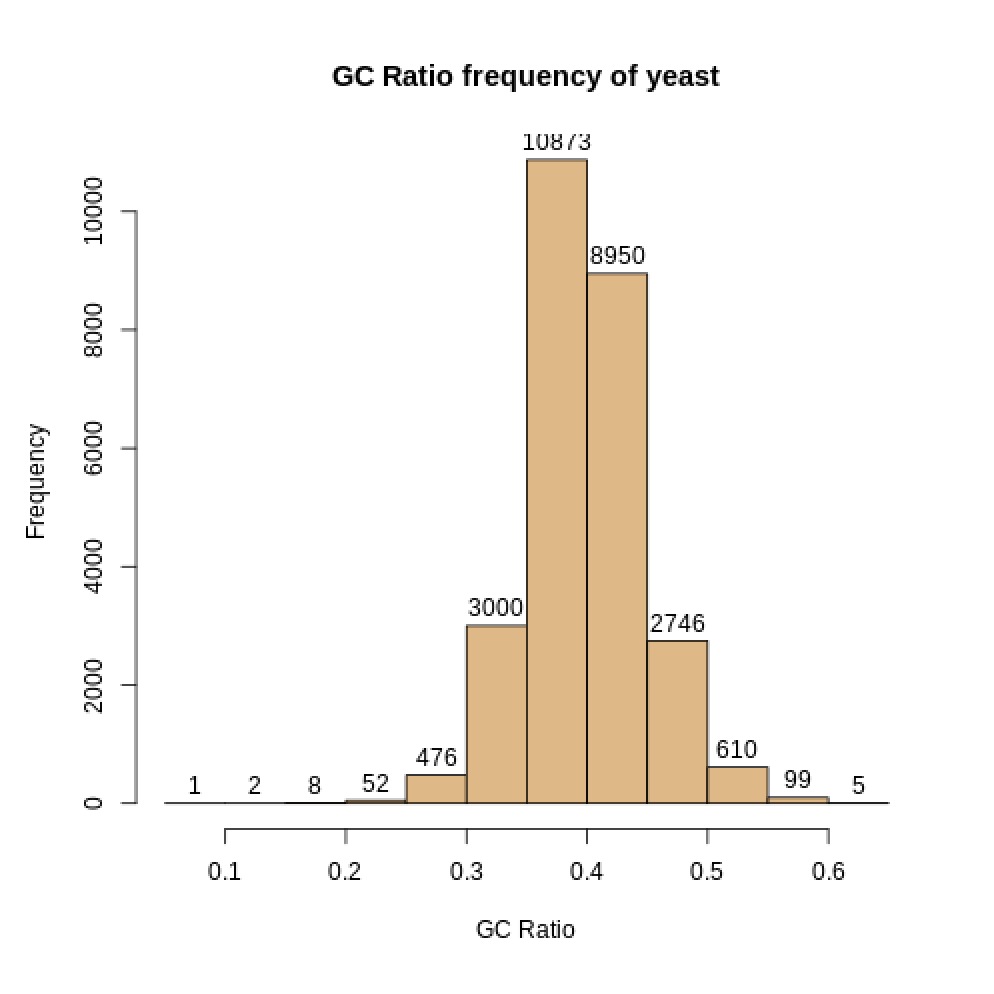
\includegraphics[width=50mm]{images/AllGenomes.eps}
\end{minipage}
\end{frame}

%------------------------------------------------

\begin{frame}
\Huge{\centerline{Thank you for attention}}
\end{frame}

%----------------------------------------------------------------------------------------

\end{document} 
